\documentclass[a4paper,12pt]{article}
\usepackage{pgfplots}
\usepackage{amsmath}
\usepackage{float}
\usepackage{multirow}
\pgfplotsset{compat=1.18}
\pagestyle{empty}
\parindent 4px
\begin{document}
\title{Planck's Constant and Inverse Square Law}
\author{Aditya Raj}
\date{Session 2024-25}
\maketitle

\section{Aim}
Determination of Planck's Constant and Verification of Inverse Square Law

\section{Apparatus Required}
\begin{itemize}
    \item Light with intensity adjustment knob
    \item Uninterrupted power supply
    \item Vaccum photo tube
    \item Colour filters 
\end{itemize}

\section{Theory}
The electromagnetic radiation consists of quanta of energy,
\begin{equation}
    \label{Planck}
    E = h \nu ,
\end{equation}
where \(E\) is energy, \(h\) is Planck's constant (to be determined) and \(\nu\) is the frequency of radiation.
These quanta are called photons. Further, it is assumed that electrons are bound inside the metal surface with an energy \(W\)
, which is called work function of that particular metal. It then follows that if frequency of the light is such that
\(h \nu > W \), it will be possible to eject photoelectron, while if \(h \nu < W \), it will not be possible.

In the former case, the excess energy of photons appears as \emph{kinetic energy} of the phototelectrons, so that
\begin{equation}
    \label{kinetic}
    \frac{1}{2}mv^2 = h \nu - W
\end{equation}
where \(m\) is mass of photoelectron and \(v\) is velocity of photoelectron.

If we can apply a retarding potenial \(V_0\) to stop the photoelectrons completely, then it is known as the \emph{stopping potenial} \(V_s\). At that instant
\begin{equation}
    \label{potenial_kinetic}
    \frac{1}{2}mv^2 = e V_s
\end{equation}
and
\begin{equation}
    \label{potential_workfunction}
    e V_s = h \nu - W
\end{equation}
where \(e\) is electron's charge equal to \(1.6 \times 10^{-19}\) , \(V_s\) is in Watts and \(W\) is in Joules.

\noindent So, when we plot graph \(V_0\) as function of \( \nu \) , the slope of straight line yields \(h\) and the intercept of extrapolated point at \(\nu = 0\) gives \(-W\).
So one can calculate value of Planck's constant and work function from the slope and intercept of the graph. \(\nu_0\) is the threshold frequency; radiation of frequency
lower than that would not help electrons to come out of surface.

If \(L\) is the luminous intensity of an electric lamp and \(E\) is the \emph{illuminiscence}, intensity of illumination at a distance \(r\) from it, then according 
to inverse square law
\begin{equation}
    \label{inverse}
    E \propto \frac{1}{r^2}
\end{equation}
If this light is allowed to fall on the cathode of a photo electric cell, then the photo electric current \(I\) would be proportional to \(E\).
\[E = \frac{L}{r^2} = kI\] Hence, a graph between \(I\) and \(\frac{1}{r^2}\) is a straight line passing though the origin, which verifies \emph{the inverse square law of radiation}.

\begin{center}
    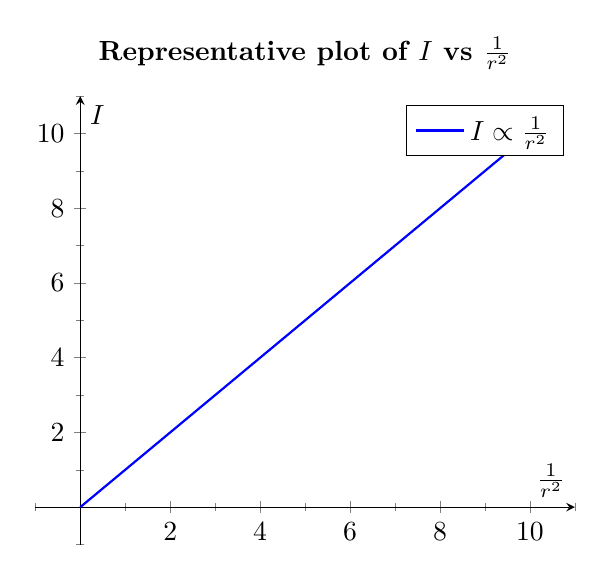
\begin{tikzpicture}
        \begin{axis}[
            xlabel = {$\frac{1}{r^2}$},
            ylabel = {$I$},
            title = {\bfseries Representative plot of $I$ vs $\frac{1}{r^2}$},
            grid = none,
            minor tick num = 1,
            xmin = 0, xmax = 10, % Set the x-axis limits
            ymin = 0, ymax = 10, % Set the y-axis limits
            axis lines = middle, % Draw axes in the middle
            enlargelimits, % Automatically enlarge limits to fit the plot
            ]
            \addplot[blue, thick, domain = 0:10]{x};
            \addlegendentry{$I \propto \frac{1}{r^2}$}
        \end{axis}
    \end{tikzpicture}    
\end{center}

\section{Tables}
\begin{table}[H]
    \def\arraystretch{2}
    \begin{center}
        \caption{Determination of Planck's constant and Work function}
        \begin{tabular}{|c|c|c|c|}
            \hline
            Colour & Wavelength (in nm) & Frequency\(\times \frac{1}{10^{14}}\) (in \(sec^{-1}\))& Stopping Potential \(V_s\) (in V)\\
            \hline
            Red & 640 & 4.6 & \(r_{10cm} = 0.077 ,\hspace{2px} r_{20cm} = 0.146\)\\
            \hline
            Orange & 670 & 5.2 & \(r_{10cm} = 0.172 ,\hspace{2px} r_{20cm} = 0.198\)\\
            \hline
            Green & 500 & 6 & \(r_{10cm} = 0.205 ,\hspace{2px} r_{20cm} = 0.255\)\\
            \hline
            Blue & 405 & 7.4 & \(r_{10cm} = 0.245 ,\hspace{2px} r_{20cm} = 0.341\)\\
            \hline
        \end{tabular}
    \end{center}
\end{table}

\begin{table}[H]
    \def\arraystretch{2}
    \begin{center}
        \caption{Calculation of Planck's constant from graph}
        \begin{tabular}{|c|c|c|}
            \hline
            Slope, \(\frac{\Delta V_s}{\Delta \nu}\) (in V.s) & Planck's constant, \(e \times slope\) (in J.s) & Mean value \(h = (h_1 + h_2)/2\) \\
            \hline
            \(m_1 = 1.37\) & \(h_1 = 2.192\) & \multirow{2}{*}{\(h_{avg} = 2.28\)} \\
            \cline{1-2}
            \(m_2 = 1.48\) & \(h_2 = 2.368\) & \\
            \hline
        \end{tabular}
    \end{center}
\end{table}

\begin{table}[H]
    \def\arraystretch{2}
    \begin{center}
        \caption{Calculation of Work function from graph}
        \begin{tabular}{|c|c|c|}
            \hline
            Intercept, \(\frac{W}{e}\) (in J/s) & Work function, \(e \times intercept\) (in J) & Mean value \(W = (W_1 + W_2)/2\) \\
            \hline
            \(c_1 = 0.230\) & \(W_1 = 0.368\) & \multirow{2}{*}{\(W_{avg} = 0.344\)} \\
            \cline{1-2}
            \(c_2 = 0.200\) & \(W_2 = 0.320\) & \\
            \hline
        \end{tabular}
    \end{center}
\end{table}

\begin{table}[H]
    \def\arraystretch{2}
    \begin{center}
        \caption{Verification of inverse square law of radiation}
        \begin{tabular}{|p{1.25in}|c|c|c|}
            \hline
            \multicolumn{2}{|c|}{Position of lamp and photo -cell} & \multicolumn{2}{|c|}{Current (\(\mu A\))}\\
            \hline
            Distance between lamp and photo cell (\(r\) in cm) & \(\frac{1}{r^2} \times 10^3\) (in \(cm^{-2}\)) & Filter: Green & Filter: Orange \\
            \hline
            5 & 40 & 0.55 & 0.51 \\
            \hline
            7 & 20 & 0.40 & 0.44 \\
            \hline
            9 & 12 & 0.30 & 0.35 \\
            \hline
            11 & 8 & 0.24 & 0.28 \\
            \hline
            13 & 5 & 0.18 & 0.22 \\
            \hline
            15 & 4 & 0.15 & 0.18 \\
            \hline
        \end{tabular}
    \end{center}
\end{table}

\section{Final Result}
So the value of Planck's constant is \(2.28 \times 10^{-34} \) J.s .\\
Work function of the material is 0.344 J.
\section{Error Calculation}
We know the value of Planck's constant is \(6.626 \times 10{-34}\) J.s (\(h\)). In our experiment, the value comes out to be \(2.28 \times 10{-34}\) J.s (\(h_{exp)}\).
So, percentage error,
\begin{align*}
    \%\, error &=  \frac{h - h_{exp}}{h} \times 100\\
    &= \frac{6.62 \times 10^{-34} - 2.28 \times 10^{-34}}{6.62 \times 10^{-34} } \times 100\\
    &= 65.5 \%
\end{align*}
\end{document}